\section{Overview}

The experiments run for a period of 100 days, from the August 1st 2013 to November 9th, 2013. During this period, we collected 9.5 GB of raw HTTP requests, consisting in approximately 11.0M GET and 1.9M POST. Our honeypots were visited by more than 73,000 different IP addresses, spanning 178 countries and presenting themselves with more than 11,000 distinct User-Agents. This is over one order of magnitude larger than what has been observed in the previous study by John et al. on low interaction web-application honeypots \cite{johnhsh}. Moreover, we also extracted over 110,000 files that were uploaded or modified during attacks against our web sites, 85,000 of them are unique.
There are two different ways to look at the data we collected: one is to identify and study the attacks looking at the web server logs, and the other one is to try to associate a goal to each of them by analyzing the uploaded and modified files. In the first part of this chapter we will look at the first part, while in the second we will give some examples of uploaded files, in order to understand attacker's goals.

\textcolor{blue}{NOTE: maybe remove Overview, as it's closed in itself (we are starting with another section for obtaining nice subsections based on the different phases)}

\section{Exploitation and Post-Exploitation Behaviors}

While analyzing the behavior of attackers lured by our honeypots, we identified four different phases commonly present in an attack session: discovery, reconnaissance, exploitation, and post-exploitation. The \emph{Discovery} phase describes how attackers find their targets, e.g. by querying a search engine (using a dork) or by simply scanning IP addresses. The \emph{Reconnaissance} phase contains information related to the way in which the pages were visited, for instance by using automated crawlers or by manual access, and if this manual access is performed via visual browser or command line tool, and if the attacker is using an anonymization proxy. In the \emph{Exploitation} phase we describe the number and types of actual attacks performed against our web applications. Some of the attacks reach their final goal themselves (for instance by changing a page to redirect to a malicious website), while others are only uploading a second stage. In this case, the uploaded file is often a web shell that is later used by the attacker to manually log in to the compromised system and continue the attack. We refer to this later stage as the \emph{Post-Exploitation} phase.

It must be noticed, however, that not all phases are present in every attack: some of them can be joined in one step (e.g., reconnaissance and exploitation are often performed in one single action), some of them are simply not present (e.g, post-exploitation), some visits do not lead to an actual attack (error in attackers requests, or incomplete file upload), and sometimes it is just impossible to link together different actions performed by the same attacker with different IP addresses.

Neverthless, by extracting the most common patterns from the data collected at each stage, we can identify the ``typical attack profile'' observed during our experiments with the following sequence:

\begin{enumerate}
\item
69.8\% of the attacks start with a scout bot visiting the page. The scout often tries to hide its User Agent (removing directly the header) or disguise themselves as a crawler search (the most used being \emph{GoogleBot});
\item
Few seconds after the scout has identified the page as an interesting target, a second automated system (hereinafter exploitation bot) visits the page and executes the real exploit. This is often a separate script that does not fake the user agent, therefore often appearing with strings such as \emph{libwww/perl}.
\item
If the vulnerability allows the attacker to upload a file, in 46\% of the cases the exploitation bot uploads a web shell. Moreover, the majority of the attacks upload the same file multiple times (in average 9, and sometimes up to 40), probably to be sure that the attack was successful.
\item
After an average of 3 hours and 26 minutes, the attacker logs into the machine using the previously uploaded shell. The average login time for an attacker interactive session is 5 minutes and 37 seconds.
\end{enumerate}

While this represents the most common behavior extracted from our dataset, many other combinations were observed as well - some of which are described in the rest of the section. Finally, it is important to mention that the attack behavior may change depending on the application and on the vulnerability that is exploited. Therefore, we should say that the previous description summarizes the most common behavior of attacks against osCommerce 2.2 (the web application that received by far the largest number of attacks among our honeypots). A particular notice must be performed regarding the SMF application: this application suffered from heavy traffic, provoked by automated bots, and we preferred to exclude this application from our statistics in order to produce more reliable results. A specific discussion over the content of messages posted on the forum will be performed later. In Figure ~\ref{fig:overview_phases} we show an overview of the four phases and its characteristics.

\begin{figure}[tbh]
\centerline{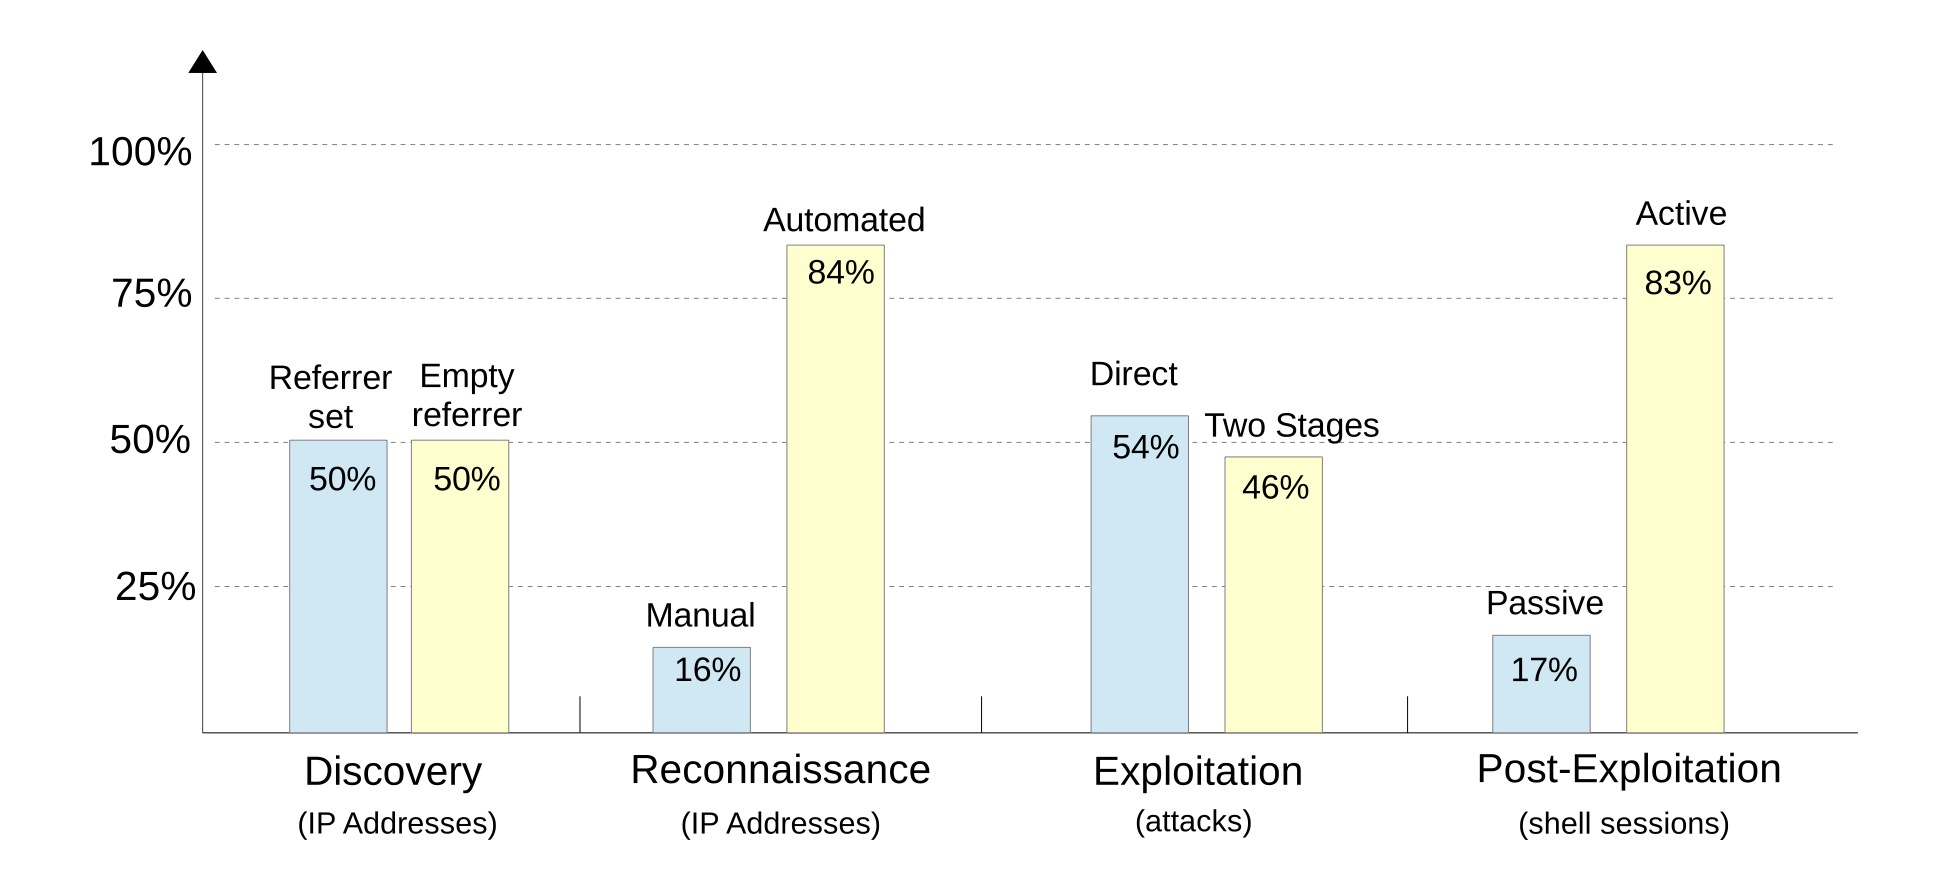
\includegraphics[scale=0.4]{Images/overview_phases.jpg}}
\caption{Overview of the four phases of an attack\label{fig:overview_phases}}
\end{figure}

\subsection{Discovery}
The very first HTTP request hit our HoneyProxy only 10 minutes after the deployment, from ``Googlebot''. The first request not related to a benign crawler came after 1 hour and 50 minutes.
During the first few days, most of the traffic was caused by benign web crawlers. Therefore, we designed a simple solution to filter out benign crawler-generated traffic from the remaining traffic. Since HTTP headers alone are not trustable (e.g., attackers often use User Agents such as ``Googlebot'' in their scripts) we collected public information available on bots and we combined them with information extracted from our logs and validated with WHOIS results in order to identify crawlers from known companies. By combining User Agent strings and the IP address ranges associated to known companies, we were able to identify with certainty 14 different crawlers, originating from 1965 different IPs. Even though this is not a complete list, it was able to successfully filter out most of the traffic generated by benign crawlers.

\begin{figure}[tbh]
\centerline{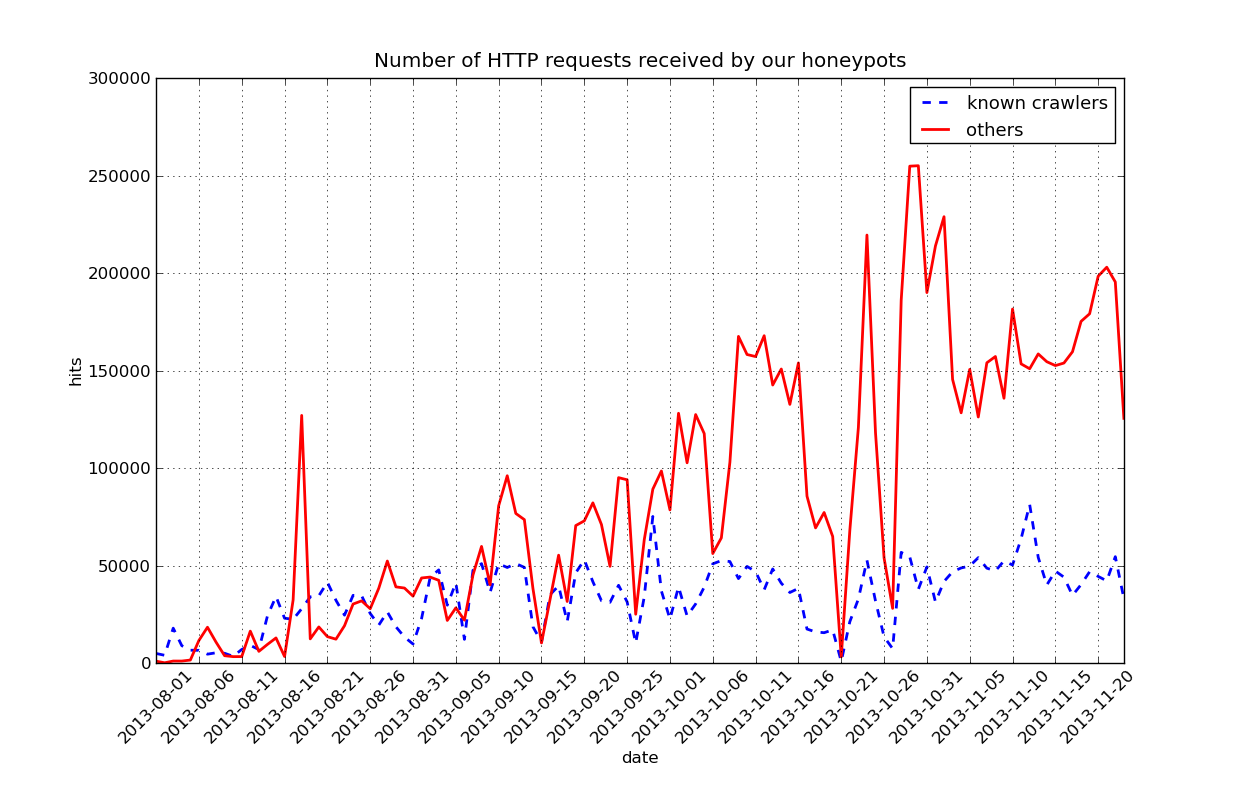
\includegraphics[scale=0.4]{Images/requestsCrawlers.png}}
\caption{Overview of the four phases of an attack\label{fig:requestsCrawlers}}
\end{figure}

Some statistics about the origin of the requests is shown in Figure ~\ref{fig:requestsCrawlers}. The amount of legitimate crawler requests is more or less stable in time, while, as time goes by and the honeypot websites get indexed by search engines and linked on hacking forums or on link farming networks, the number of requests by malicious bots or non-crawlers has an almost linear increase.
While looking at these statistics we also noticed a number of suspicious spikes in the number of accesses. In several cases, one of our web applications was visited, in few hours, by several thousands of unique IP addresses (compared with an average of 192 per day), a clear indication that a botnet was used to scan our sites.

Interestingly, we observed the first suspicious activity only 2 hours and 10 minutes after the deployment of our system, when our forum web application started receiving few automated registrations. However, the first posts on the forum appeared only four days later, on December 27th. Even more surprising was the fact that the first visit from a non-crawler coincided with the first attack: 4 hours 30 minutes after the deployment of the honeypots, a browser with Polish locale visited our osCommerce web application and exploited a file upload vulnerability to upload a malicious PHP script to the honeypot. We also examined the IP source address in order to understand the more active countries, as we can see from ~\ref{fig:requests_countries} China, Russia, and USA are in order the top three countries for number of requests. \textcolor{blue}{HEATMAP OR PIE CHART?}.

\begin{figure}[tbh]
\centerline{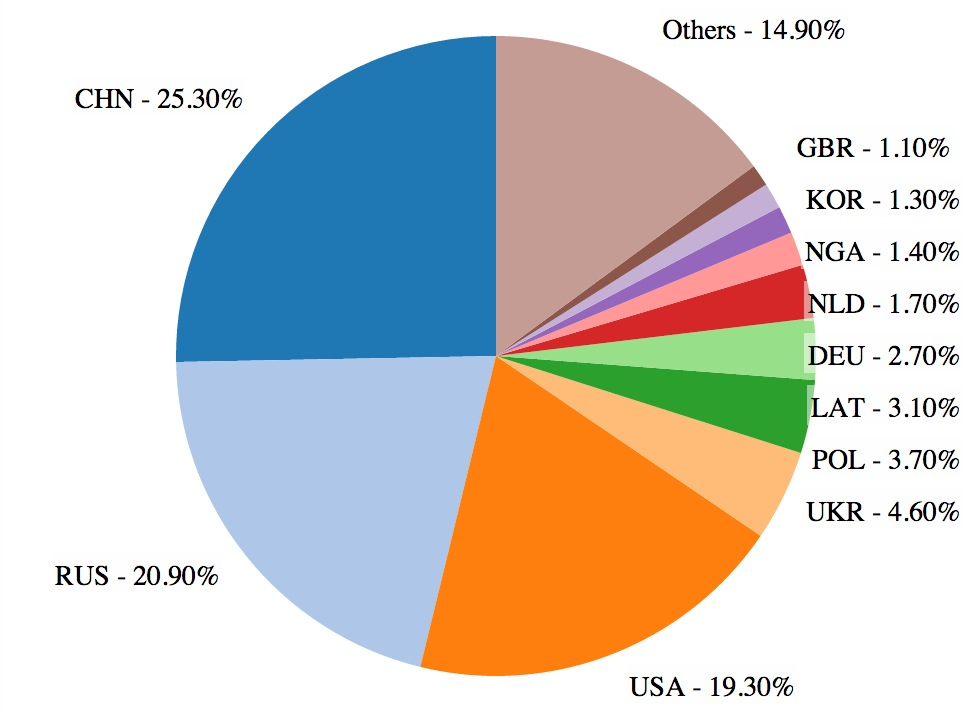
\includegraphics[scale=0.5]{Images/requests_countries.jpg}}
\caption{Number of requests divided by country\label{fig:requests_countries}}
\end{figure}

\subsubsection{Referer Analysis}

The analysis of the Referer HTTP header (whenever available) helped us identify how visitors were able to find our honeypots on the web. Based on the results, we can distinguish two main categories of users: attackers using search engines to find vulnerable applications, and victims of phishing attacks following links posted in emails and public forums.
A total of 66,449 visitors reached our honeypot pages with the Referer header set. The domains that appear most frequently as referrers are search engines, followed by web mails and public forums. Google is leading with 17,156 entries. Other important search engines used by the attackers to locate our websites, were Yandex (1,016), a russian search engine, Bing (263), Microsoft search engine, and Yahoo (98). A total of 7,325 visitors arrived from web mail services (4,776 from SFR, 972 from Facebook, 944 were from Yahoo! Mail, 493 from Live.com, 407 from AOL Mail, and 108 from comcast.net). Finally, 15,746 requests originated from several public web forums, partially belonging to hacking communities, and partially just targeted by spam bots.

Finally, we extracted search queries (also known as ``dorks'', when used for malicious purposes) from Referer headers set by the most common web search engines. Our analysis shows that the search terms used by attackers highly depend on the application deployed on the honeypot. For example, the most common dork that was used to reach our Joomla web application contained the words \emph{``joomla allows you''}, while the Simple Machines Forum was often reached by searching \emph{``powered by smf''}. Our machine containing public web shells was often reached via dorks like \emph{``inurl:c99.php''}, \emph{``cyber anarchy shell''} or even \emph{``ftp AND brute-forcer AND security AND info AND processes AND mysql AND php-code AND en-coder AND backdoor AND back-connection AND home AND enumerate AND md5-lookup AND word-lists AND milw0rm AND itsearch AND self-kill AND about''}. The latter query, even though very long, was used more than 150 times to reach our machine with web shells. It was probably preferred to searching via \emph{``intitle:''} or \emph{``inurl:''} because attackers tend to customize names and titles of the scripts, therefore a search for direct text content may return more results. Some specialized search engines appear to be used as well, such as devilfinder.com \cite{devilfinder}, which was adopted in 141 cases to reach some of the shells on our machines. This search engine claims to show more low-ranking results than common search engines, not to store any search data, and to return up to 300 results on the same web page, making it very suitable for attackers willing to search for dorks and collect long lists of vulnerable websites.

\subsection{Reconnaissance}

After removing the legitimate crawlers, the largest part of the traffic received by our honeypots was from unidentified sources, many of which were responsible of sending automated HTTP requests. We found these sources to be responsible for the majority of attacks and spam messages targeting our honeypots during our experiments.

However, distinguishing attackers that manually visited our applications from the ones that employed automated scout bots is not an easy task. We applied the following three rules to flag the automated requests:

\begin{description}
\item[Inter-arrival time.] If requests from the same IP address arrive at a frequency higher than a certain threshold, we consider the traffic as originated from a possible malicious bot.
\item[Request of images.] Automated systems, and especially those having to optimize their speed, almost never request images or other presentation-related content from websites. Scanning web logs for visitors that never request images or CSS content is thus an easy way of spotting possible automated scanners.
\item[Subdomain visit pattern.] As described in Chapter 1, each web site we deployed consisted in a number of subdomains linked together according to a predetermined pattern. If the same IP accesses them in a short time frame, following our patterns, then it is likely to be an automated crawler.
\end{description}

For example, after removing the benign crawlers, a total of 9.5M hits were received by systems who did not request any image, against 1.8M from system that also requested images and presentation content. On the contrary, only 641 IP addresses (responsible for 13.4K hits) visited our websites by following our links in a precise access pattern. Among them, 60\% followed a breadth first approach.
85\% of the automated requests were directed to our forum web application, and were responsible for registering fake user profiles and posting spam messages. Of the remaining 1.4M requests directed to the seven remaining honeypot applications, 95K were mimicking the User-Agent of known search engines, and 264K switched between multiple User-Agents over time. The remaining requests did not contain any suspicious User-Agent string, did not follow paths between domains, neither requested images. As such, we classified them as unknown (possibly benign) bots.

\subsection{Exploitation}

The first important activity we performed in order to detect exploitation attempts was parsing the log files in search of attack traces. Luckily, knowing already the vulnerabilities affecting our web applications allowed us to quickly and reliably scan for attacks in our logs using a set of regular expressions.
Overall, we logged 444 distinct exploitation sessions. An interesting finding is that 310 of them adopted two or more different User-Agent strings, appearing in short sequence from the same IP address. As explained before, this often happens when attackers employ a combination of scout bots and automatic attack scripts in order to speed up attacks and quickly find new targets. In particular, in two thirds (294) of the total exploitation sessions we observed, the User-Agent used for the exploitation was the one associated to the LibWWW Perl library (libwww/perl).
In some of these exploitation sessions, the attacker tried to disguise her tools and browser as known benign bots. Some crawler User-Agent strings that were often used during exploitation sessions were: FreeWebMonitoring, Gigabot/3.0, gsa-crawler, IlTrovatore-Setaccio/1.2, bing- bot/2.0;, and Googlebot/2.1.

\begin{figure}[tbh]
\centerline{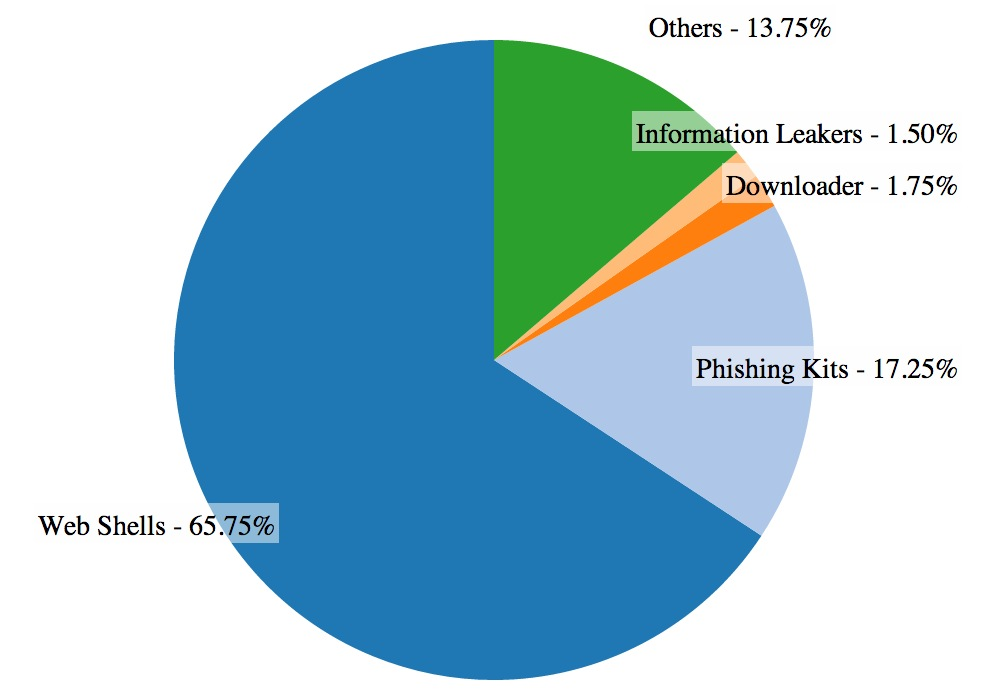
\includegraphics[width=0.7\textwidth]{Images/1stStageAttack.jpg}}
\caption{1st Stage attack file categorization.\label{fig:1stStageAttack}}
\end{figure}

The most remarkable side effect of every exploitation session is the upload or modification of files on the victim machine. Quite surprisingly, we noticed that when an exploitation session uploads a file, the file is uploaded in average 9.75 times. This strange behavior can be explained by the fact that most of the exploitation tools are automated, and since the attacker does not check in real-time whether each exploit succeeded or not, uploading the same file multiple times can increase the chance for the file to be successfully uploaded at least once. Results of this phase, resumed in Figure~\ref{fig:1stStageAttack}, show that the files uploaded during attack sessions consist, in 65.75\% of the cases, in web shells, in 17.25\% of the cases in phishing files (single HTML pages or complete phishing kits), in 1.75\% of the cases in scripts that automatically try to download and execute files from remote URLs, and in 1.5\% of the cases in scripts for local information gathering. The remaining 13.75\% of the files include malwares, defacement pages and several other categories.

\begin{figure}[tbh]
\centerline{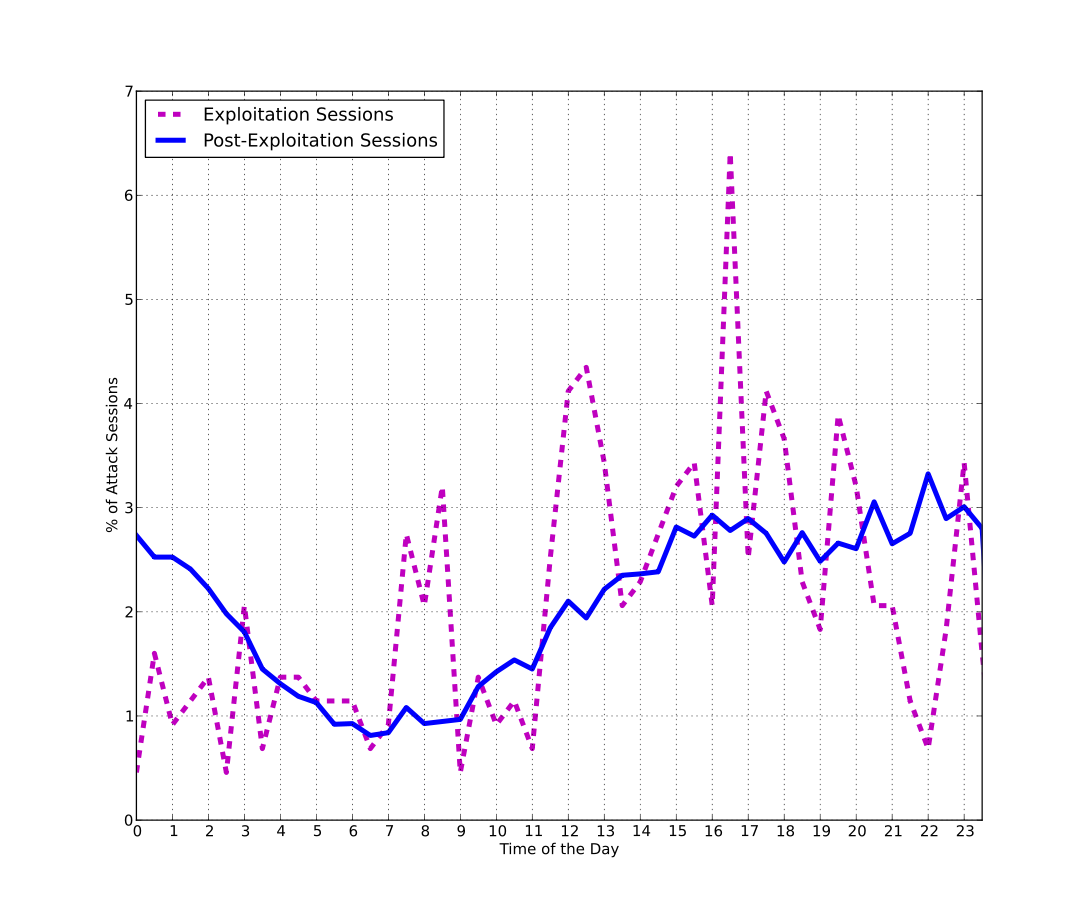
\includegraphics[width=0.7\textwidth]{Images/normalizedAttackTimes.png}}
\caption{Normalized time of attack sessions.\label{fig:normalizedAttackTimes}}
\end{figure}

Figure~\ref{fig:normalizedAttackTimes} shows the normalized times of the attacks received by our honeypots. The values were computed by adjusting the actual time of the attack with the timezone extracted from the IP geolocalization. It must be noticed that, using this method, we can have some false values in case the attacker is proxying its connection through an IP in a different part of the world. However, the graph shows a clear daylight trend for both the exploitation and post-exploitation phases. In particular, for the interactive sessions we observed fewer attacks performed between 4am and 10am, when probably also the criminals need to get some sleep. Interestingly, also the exploitation phase, that is mostly automated, shows a similar trend (even though not as clear). This could be the consequence of scans performed by botnet infected machines, some of which are probably turned off by their users during the night.

\subsubsection{Forum Activity}

Since the 1st day of operation, our forum application received a very large amount of traffic. Most of it came from automated spamming bots that kept flooding the forum with fake registrations and spam messages. We analyzed every snapshot of the machine's database in order to extract information about the forum's posts and the URLs that were embedded in each of them. This allowed us to identify and categorize several spam and link farming campaigns, as well as finding some rogue practices such as selling forum accounts.

A total of 68,201 unique messages were posted on the forum during our study, by 15,753 users using 3,144 unique IP addresses. Daily statistics on the forum show trends that are typical of medium to high traffic message boards: an average of 604 posts per day (with a max of 3085), with an average of 232 online users during peak hours (max 403).
Even more surprising than the number of posts is the number of new users registered to the forum: 1907 per day in average, and reaching a peak of 14,400 on October 23, 2013. We measured that 33.8\% of the IP addresses that performed actions on our forum were responsible of creating at least one fake account, but never posted any message. This finding suggests there are some incentives for criminals to perform automatic user registrations, and perhaps selling user accounts is even more profitable than the spamming activity itself. Our hypothesis is that, in some cases, forum accounts can be sold in bulk to other actors in the black market. We indeed found 1,260 fake accounts that were created from an IP address and then used few days later by other, different IPs, to post messages. This does not necessarily validate our hypothesis, but shows at least that forum spamming has become a complex ecosystem and it is difficult, nowadays, to find only a single actor behind a spam or link farming campaign.

\begin{figure}[tbh]
\centerline{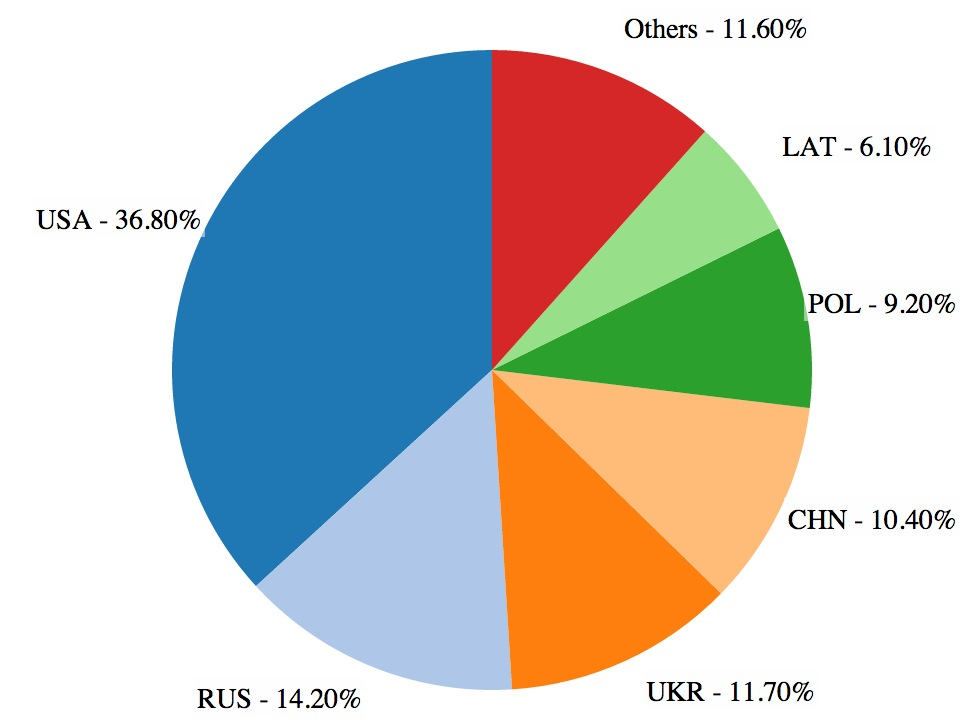
\includegraphics[width=0.7\textwidth]{Images/spamCountriesIP.jpg}}
\caption{Country provenance of IPs active on forum (message posting or registration).\label{fig:spamCountriesIP}}
\end{figure}

We tracked the geolocation of IP addresses responsible for registering users and posting to the forum. We identified the countries which are the most active on this category of rouge activity as the United States and Eastern Europe countries (mostly Russia, Ukraine, Poland, Latvia, Romania), as shown in Figure~\ref{fig:spamCountriesIP}. A total of 6687 distinct IP addresses were active on our forum (that is, posted at least one message or registered one or more accounts). Among these, 36.8\% were associated to locations in the US, while 51.6\% came from one of the cited Eastern European countries. The country coverage drastically changes if we consider only IP addresses that posted at least one message to the forum (ref Figure~\ref{fig:spamCountriesMessage}). In this case, IPs from the United States represent, alone, 62.3\% of all the IP addresses responsible for posting messages (Eastern Europe IPs in this case represent 21.2\% of the total), while we have much more variety in the number of different countries involved in the activity. This behavior strongly suggests a country-related specialization in malicious activities, where a small number of attackers in few areas sell on the black market the results of their activities to foreign agents, who perform different activities.

\begin{figure}[tbh]
\centerline{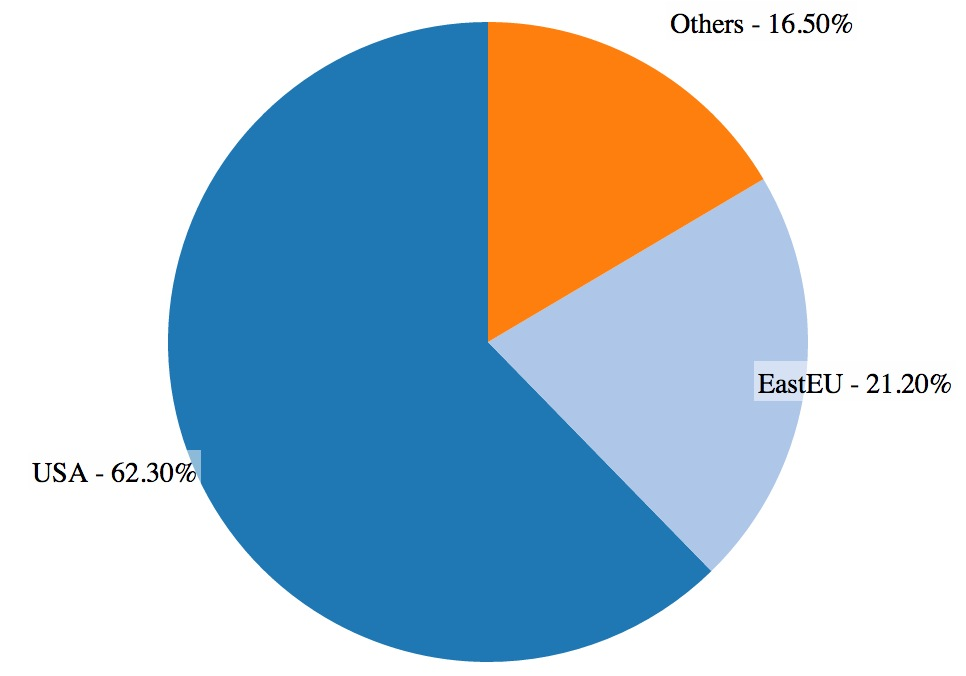
\includegraphics[width=0.7\textwidth]{Images/spamCountriesMessage.jpg}}
\caption{Country provenance of IPs posting at least one message.\label{fig:spamCountriesMessage}}
\end{figure}

Finally, we performed a simple categorization on all the messages posted on the forum, based on the presence of certain keywords. This allowed us to quickly identify common spam topics and campaigns. Thanks to this method, we were able to automatically categorize 63,763 messages (93.5\% of the total).
As shown in Figure~\ref{fig:SpamCategory}, the trends we extracted from message topics reveal that the most common category is drugs (45.2\% of the categorized messages, and showing peaks of 2000 messages per day), followed by search engine optimization (SEO, 17.4\%), electronics (13.5\%), adult content (7.9\%), and health care(5.2\%).
All the links inserted in the forum posts underwent an in-depth analysis using two automated, state-of-the-art tools for the detection of malicious web pages, namely Google Safe Browsing \cite{googleSafeBrowsing} and Wepawet \cite{wepaWet}. The detection results of these two tools show that, on the 221,423 URLs we extracted from the forum posts, a small but not insignificant fraction (2248, roughly 1 out of 100) consisted in malicious or possibly harmful links.

\begin{figure}[tbh]
\centerline{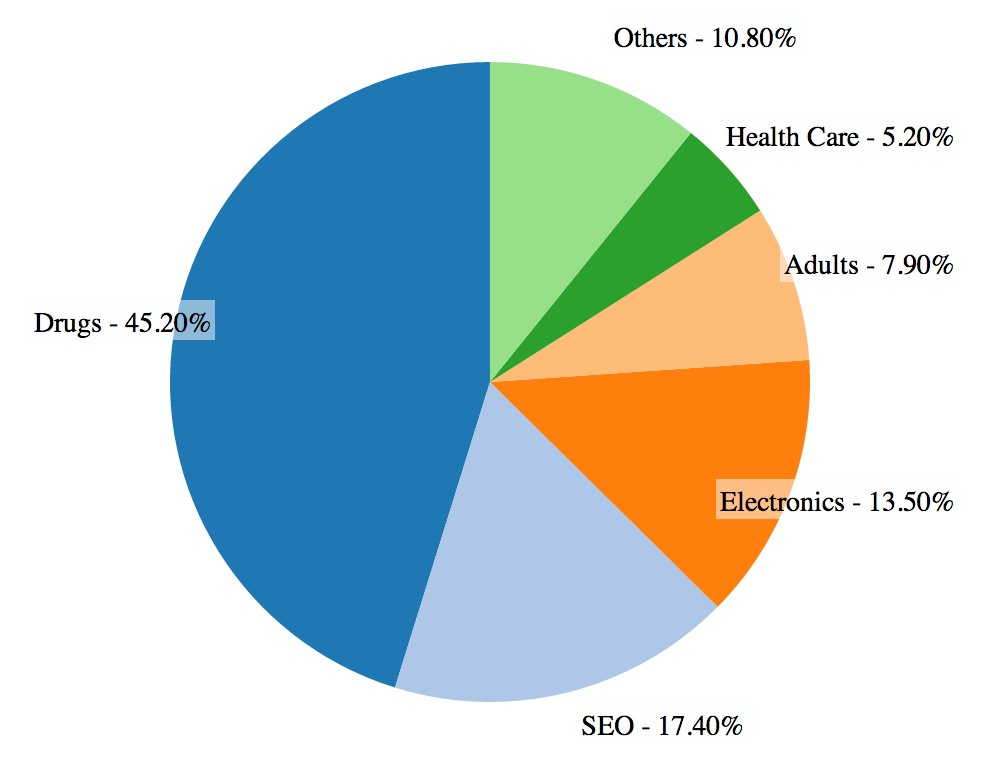
\includegraphics[width=0.7\textwidth]{Images/SpamCategory.jpg}}
\caption{Categories of spam messages.\label{fig:SpamCategory}}
\end{figure}

\subsection{Post-Exploitation}

The post-exploitation phase includes the analysis of the interaction between the attackers and the compromised machines. In our case, this is mostly done through the web shells installed during the exploitation phase or through the access to the public shells that we already pre-installed in our virtual machines.

The analysis of the post-exploitation phase deserves special attention since it is made of interactive sessions in which the attackers can issue arbitrary commands. However, these web shells do not have any notion of session: they just receive commands via HTTP requests and provide the responses in a state-less fashion. We decided to identify an ``interactive sessions'' every time a sequence of more than 3 commands is issued from the same IP and the idle time between consecutive commands is less than 5 minutes.
Over a total of 74,497 shell commands received, we registered 232 interactive sessions with an uploaded webshell and 8268 with one of our pre-installed shells. Because of the minimum number of commands threshold we imposed for the identification of a session only 52,368 shell commands have been included in a session. The majority of the commands not included in a session are single file uploads through one of our pre-installed webshells, mostly for defacement purposes.

The average session duration was of 5 minutes and 37 seconds, however, we registered 9 sessions lasting more than one hour each. The longest, in terms of commands issued to the system, was from a user in Saudi Arabia that sent 663 commands to the shell, including the manual editing of several files. Interestingly, one of the most common actions performed by users during an attack is the upload of a custom shell, even if the attacker broke into the system using a shell that was already available on the website. The reason for this behavior is that attackers know that, with a high probability, shells already installed on a system will contain backdoors and most likely leak information to their owner. In addition to the 17 web shells supported by our tools, we also identified the HTTP patterns associated to the most common custom shells uploaded by the attackers, so that we could parse the majority of commands issued to them.
In 83\% of the cases, attackers tried to use at least one active command (uploading or editing a file, changing file permissions, creating files or directories, scanning hosts, killing a process, connecting to a database, sending emails, etc.). The remaining sessions were purely passive, with the attackers only browsing our system and downloading source and configuration files.
Finally, in 61\% of the sessions the attackers uploaded a new file, and in 50\% of them they tried to modify a file already on the machine (in 13\% of the cases to perform a defacement). Regarding individual commands, the most commonly executed were the ones related to listing and reading files and directories, followed by editing files, uploading files, running commands on the system, listing the processes running on the system, and downloading files.

During this phase most of the attackers created or uploaded a new file: as can be seen in Figure~\ref{fig:2ndStageAttack}, there is much more variety in the category of files uploaded, as during this stage the attackers is trying to accomplish a certain goal rather than just obtain an access to the machine. The results do not consider attacks where a webshell is uploaded, as we still consider this action to be a 1st stage attack.

\begin{figure}[tbh]
\centerline{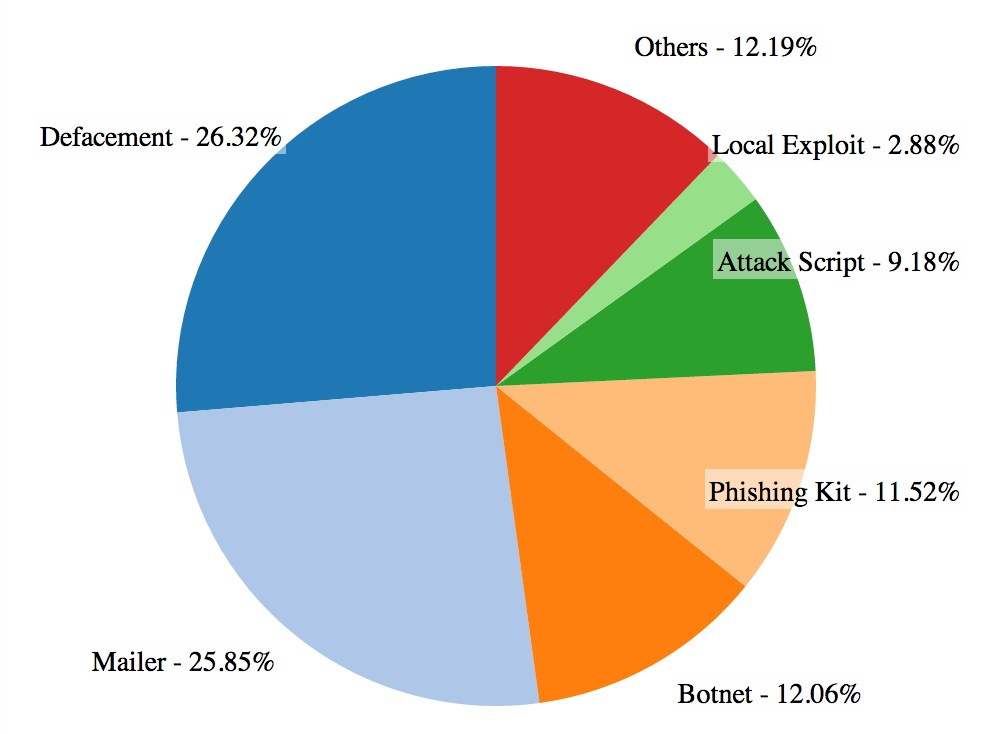
\includegraphics[width=0.7\textwidth]{Images/2ndStageAttack.jpg}}
\caption{2nd Stage Attack File Categorization\label{fig:2ndStageAttack}}
\end{figure}

It's evident how the variety of files is increased. In the next chapter we are going to explore in details attackers goals and single file categories, we provide here a first introduction to the various categories:

\begin{description}
\item[Defacement] The most common type of file uploaded, it's usually just an HTML document with the name of the attacker/team who performed the malicious activity;
\item[Mailer] A mailer is a script (usually written in PHP or Perl) for spamming purposes, it usually tries to read a list of e-mail addresses and sends the same message to each of them;
\item[Botnet] these scripts communicate with other machines for performing several tasks, transforming the hosting machine in a bot which receives and execute commands sent by others;
\item[Phishing Kit] it's a collection of HTML pages, images and CSS files, usually uploaded as compressed archives, looking like a ``famous'' website in order to fool a victim to insert their credentials. The most common copied website is Paypal, followed by Visa and FaceBook;
\item[Attack Scripts] This is a general category for including every script that is able to look for other websites and automatically exploit them. They usually accept a list of urls and, for each of them, they try to exploit a known vulnerability (like a vulnerable plugin for Joomla, etc);
\item[Local Exploits] This category relies with files that are trying to compromize the same machine they are running on, usualdly by means of privilege escalation.
\end{description}

Other categories include Uploaders, SQL dumpers, Malwares, Network Scanners, Drive-by Downloads, Flooder Scripts etc.

\section{Attackers Goals}

In this section we shift the focus from the way the attacks are performed to the motivation behind them. In other words, we try to understand what criminals do after they compromise a web application, and why. We discovered several goals attackers try to achieve after exploiting a machine: some of them are just looking for public recognition, some others are trying to create a botnet for profit, others are involved in spamming and phishing campaigns.

\begin{table}[tbh] % per piazzare la tabella t:top b:bottom h:here in ordine di preferenza; h è sconsigliato
\begin{center}
\begin{tabularx}{\textwidth}{|c|X|X|}
\hline
\textit{Category} & \textit{Unique Files} & \textit{Total Number Of Files} \\
\hline
Fake Downloads & 24 & 24 \\
Code Inclusion & 177 & 242 \\
Malicious Files Discovery & 216 & 217 \\
Java Applet & 221 & 225 \\
Drive-by Download & 284 & 310 \\
SQL dumper & 287 & 292 \\
Proxy & 335 & 343 \\
System Info Leaker & 341 & 387 \\
Mass Defacer & 356 & 383 \\
WebSearch Bot & 413 & 425 \\
Network Scanner & 420 & 445 \\
Malware & 475 & 492 \\
Documents & 516 & 518 \\
Uploader & 597 & 740 \\
Configuration Overloader & 656 & 713 \\
Backdoor & 703 & 728 \\
Bruteforcer Script & 2457 & 2659 \\
Local Exploit & 3033 & 3322 \\
Flooder Script & 3341 & 3452 \\
Attack Script (to other machines) & 4956 & 6064 \\
Botnet & 7878 & 8912 \\
Phishing Pack & 9445 & 18608 \\
Mailer & 13012 & 15324 \\
Defacement & 14698 & 18023 \\
Webshell & 20322 & 28551 \\
\hline \hline
Total & 85163 & 111399 \\
\hline
\end{tabularx}
\caption{Summary of files Received.\label{tab:webapps}}
\end{center}
\end{table}

We analyzed the files uploaded during the exploitation phase, and the ones created or modified during the post-exploitation phase. We normalized each file content, and we clustered them together according to their similarity, obtaining several clusters according to their ``purpose''. We identified a total of 25 categories, and the results are displayed in table~\ref{tab:webapps}. From the table we removed all broken files. The corresponding graphs shows the distribution of files according to their percentage.

\begin{figure}
\centering
\begin{subfigure}{.5\textwidth}
  \centering
  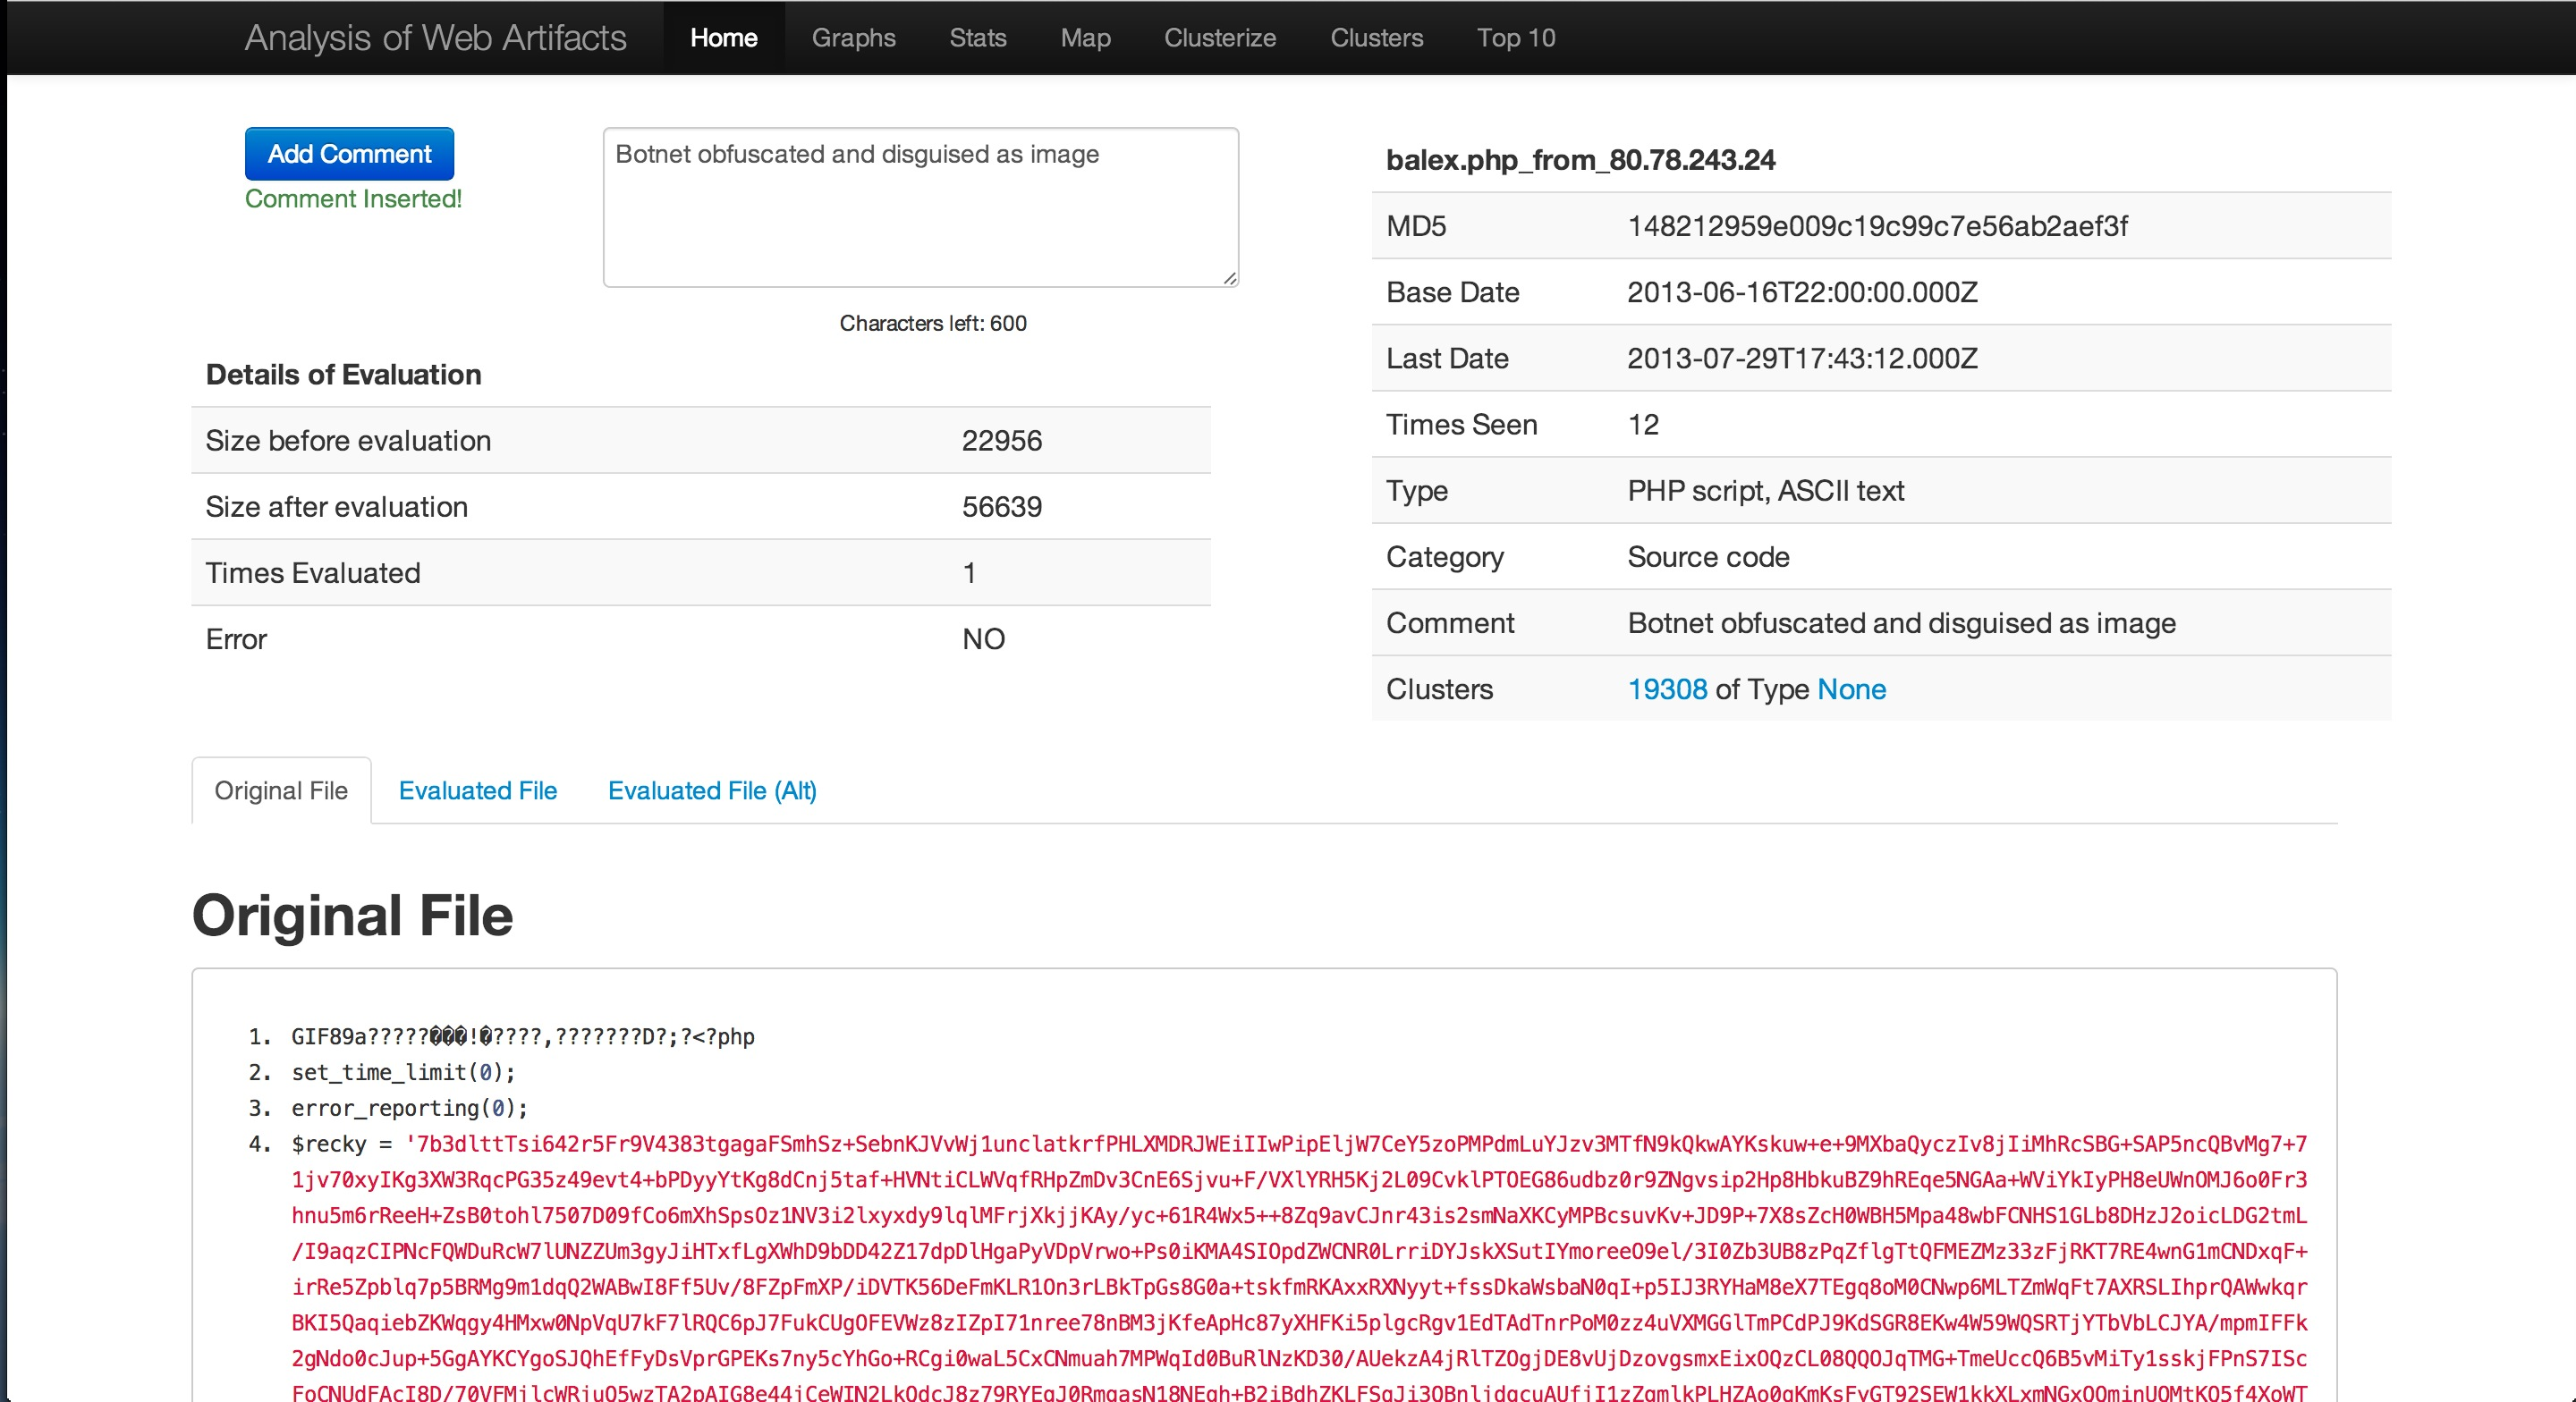
\includegraphics[width=1.0\linewidth]{Images/obf_file.jpg}
  \caption{Unique Files Distribution}
  \label{fig:sub1}
\end{subfigure}%
\begin{subfigure}{.5\textwidth}
  \centering
  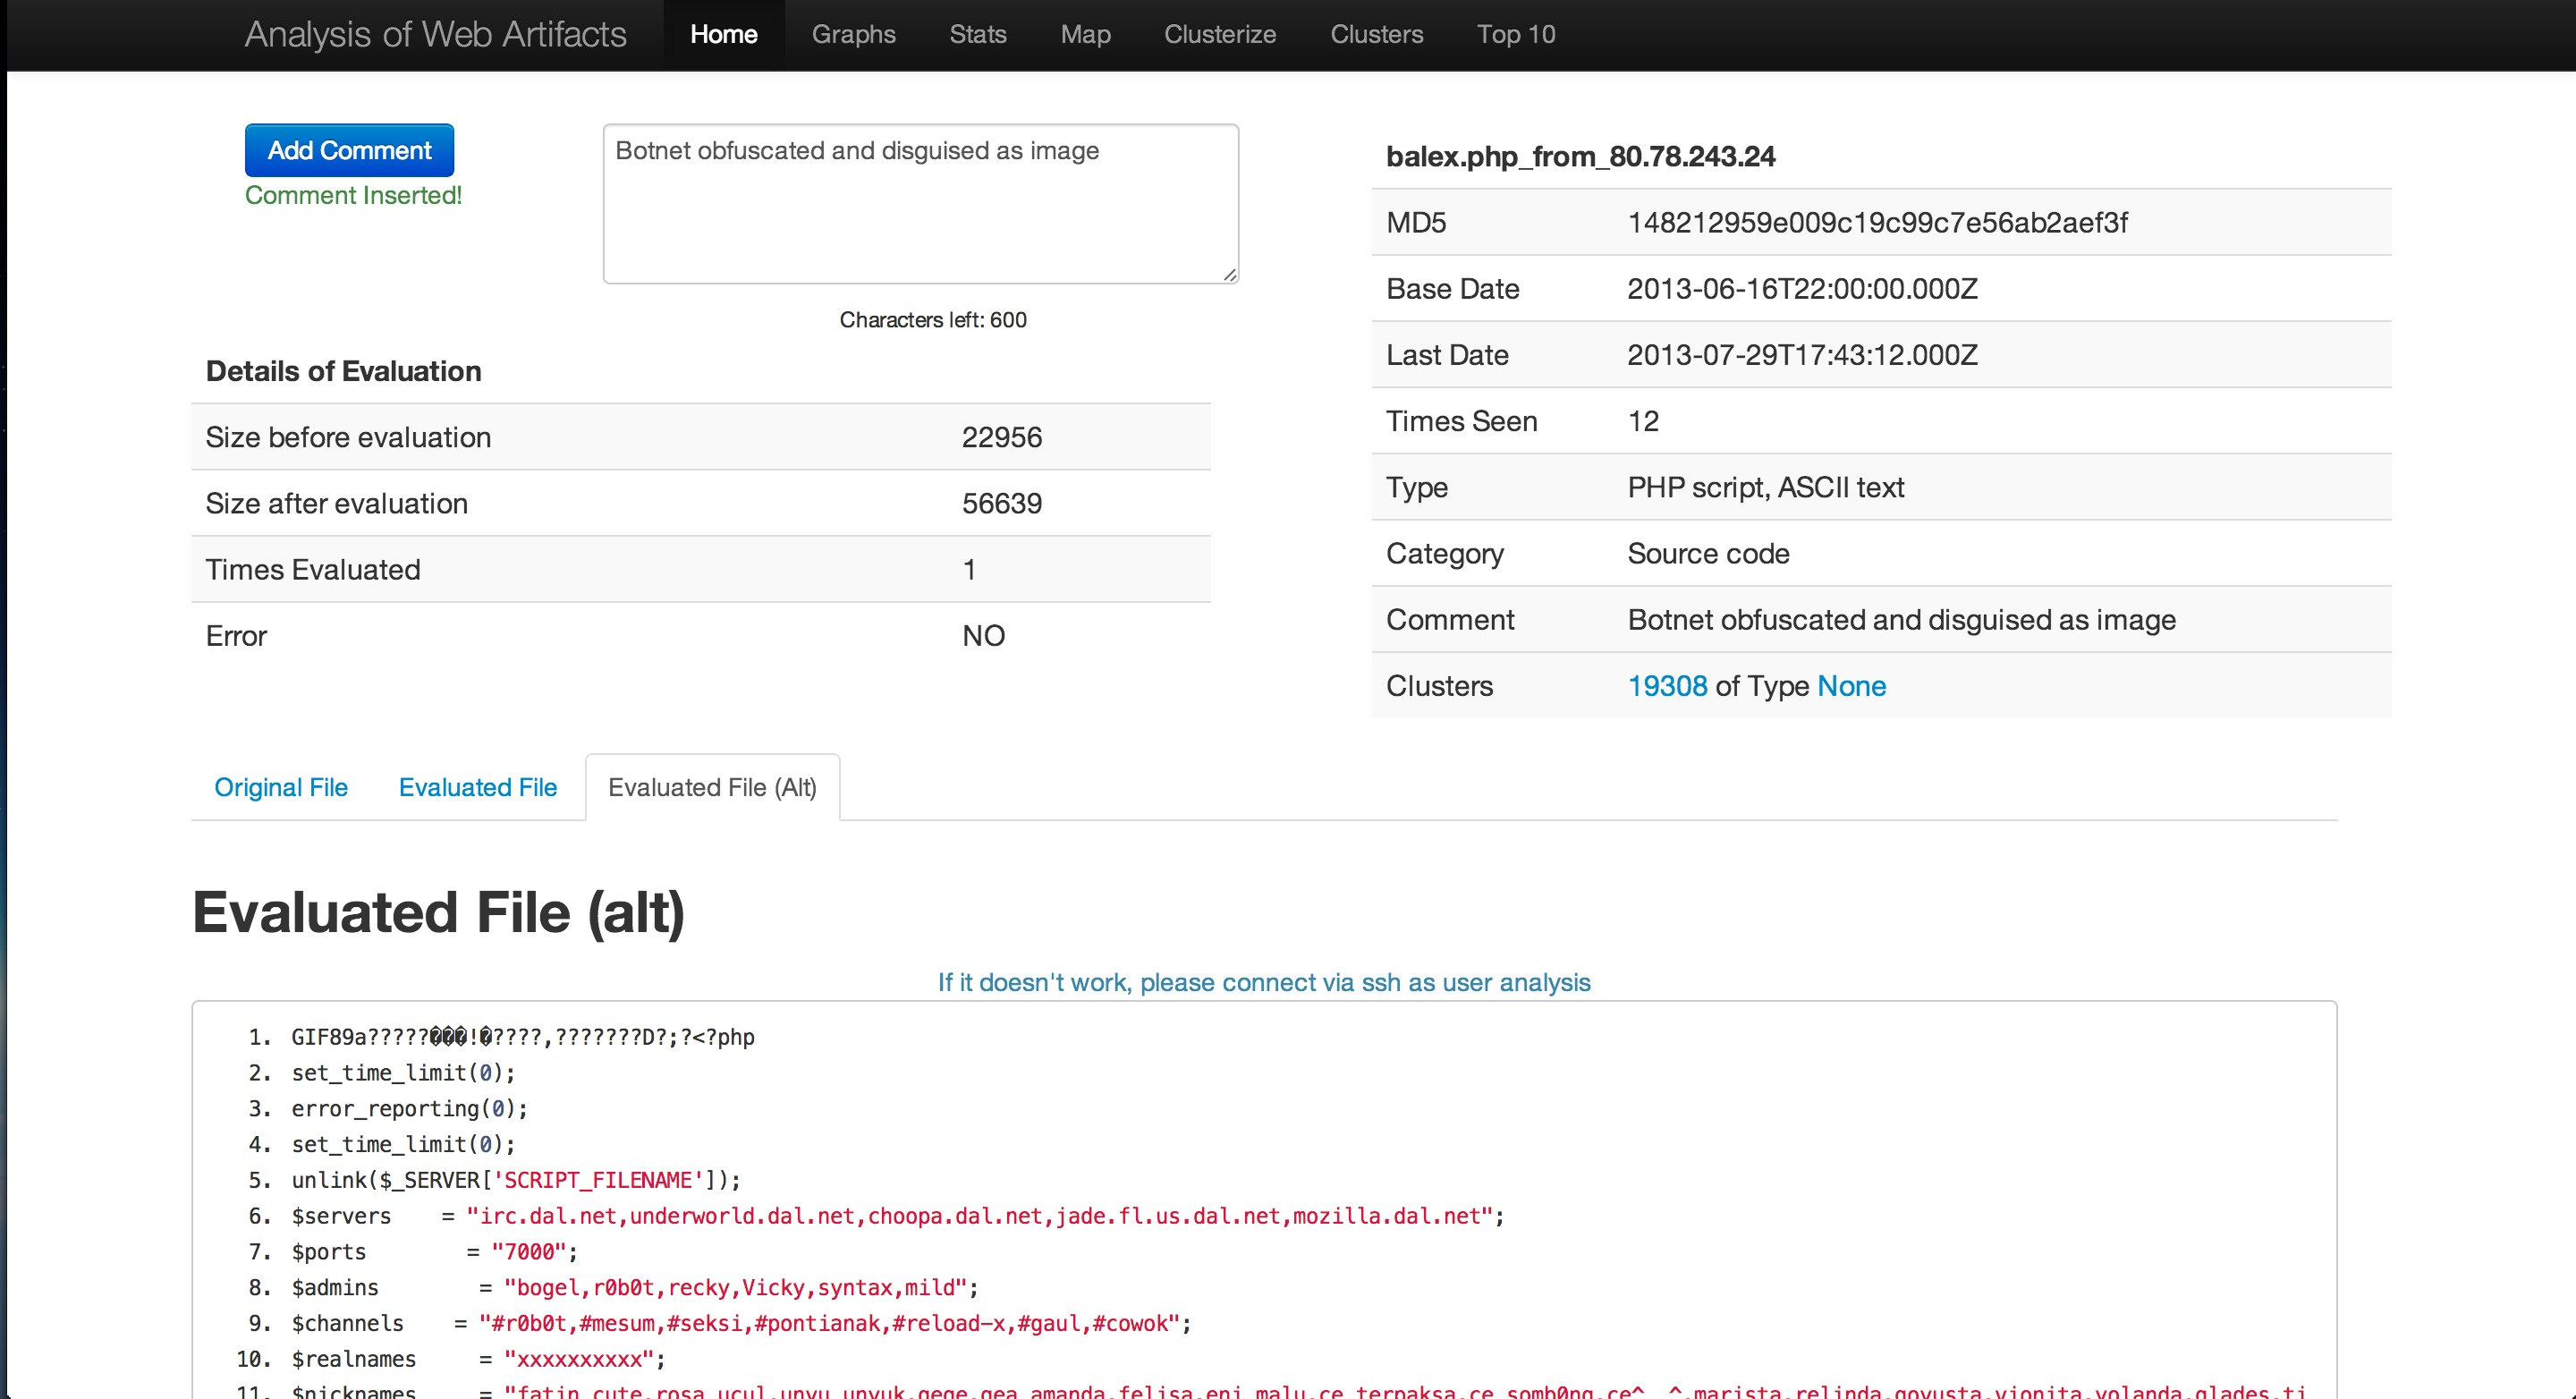
\includegraphics[width=1.0\linewidth]{Images/deobf_file.jpg}
  \caption{Total Files Distribution}
  \label{fig:sub2}
\end{subfigure}
\caption{Categorization of files received}
\label{fig:test}
\end{figure}

For example, 1.7\% of the unique files we observed in our experiments were used to try to escalate the privileges on the compromised machine. This is different from saying that 1.7\% of the attackers tried to escalate the privileges of the machine. Unfortunately, linking the files to the attacks in which they were used is not always possible. Therefore, we computed an estimation of the attackers that performed a certain action by identifying each unique IP that uploaded a certain file during an
